\section{Diagrama de Tempo (\textit{Waveform})}

\begin{frame}{Diagrama de Tempo (\textit{Waveform})}
	\par Quando fazemos o diagrama de tempo ou o \textit{waveform} apresentamos ao circuito uma sequência de  sinais de forma que o circuito responde a essa sequência gerando outras sequências. 
	\begin{itemize}
		\item Mostra os estados do circuito ao longo do tempo.
		\item Permite a visualização do comportamento do circuito durante o tempo.
	\end{itemize}
	\begin{figure}
		\centering
		\includegraphics[width=\linewidth]{images/waveform01}
		\caption{Consegue saber qual porta é esta?}
		\label{fig:waveform01}
	\end{figure}
\end{frame}

\begin{frame}{Prática dirigida 01}
	\par Construção de Circuito a partir de Expressão Algébrica
	\begin{itemize}
		\item Dada a expressão algébrica \(f(x, y, z) = \overline{x} \cdot y + x \cdot \overline{y} \cdot z\), construa: %f=(~x*y)+(x*~y*z)
		\begin{enumerate}
			\item O circuito correspondente usando portas lógicas básicas (AND, OR, NOT).
			\item A tabela verdade que representa o comportamento da função.
			\item O diagrama de tempo (waveform) que mostra os estados do circuito para todas as combinações de \(x\), \(y\) e \(z\) ao longo do tempo.
		\end{enumerate}
	\end{itemize}
	\pause
	\begin{columns}
		\column{.8\linewidth}
			\begin{figure}
				\centering
				% Important: If latex complains about unicode characters,
% please use "\usepackage[utf8x]{inputenc}" in your preamble
% You can change the size of the picture by putting it into the construct:
% 1) \resizebox{10cm}{!}{"below picture"} to scale horizontally to 10 cm
% 2) \resizebox{!}{15cm}{"below picture"} to scale vertically to 15 cm
% 3) \resizebox{10cm}{15cm}{"below picture"} a combination of above two
% It is not recomended to use the scale option of the tikzpicture environment.
 \resizebox{7cm}{!}{
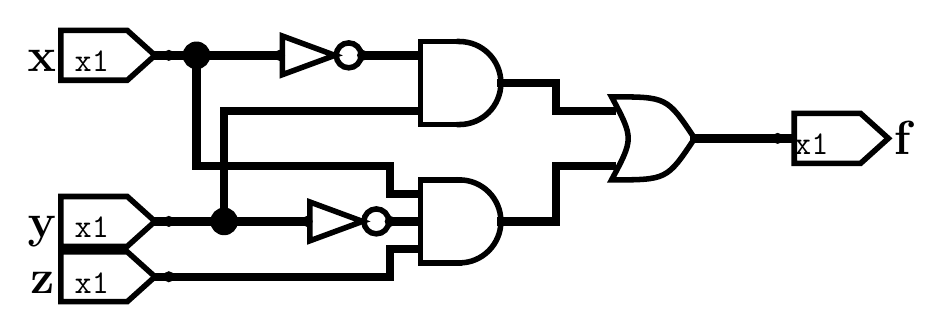
\begin{tikzpicture}[x=1pt,y=-1pt,line cap=rect]
\def\logisimfontA#1{\fontfamily{cmr}{#1}} % Replaced by logisim, original font was "SansSerif"
\def\logisimfontB#1{\fontfamily{cmtt}{#1}} % Replaced by logisim, original font was "Monospaced"
\definecolor{custcol_0_0_0}{RGB}{0, 0, 0}
\definecolor{custcol_ff_ff_ff}{RGB}{255, 255, 255}
\draw [line width=3.0pt, custcol_0_0_0 ]  (246.0,45.0) -- (276.0,45.0) ;
\draw [line width=3.0pt, custcol_0_0_0 ]  (126.0,15.0) -- (146.0,15.0) ;
\draw [line width=3.0pt, custcol_0_0_0 ]  (136.0,75.0) -- (146.0,75.0) ;
\draw [line width=3.0pt, custcol_0_0_0 ]  (96.0,15.0) -- (66.0,15.0) -- (66.0,55.0) -- (136.0,55.0) -- (136.0,65.0) -- (146.0,65.0) ;
\draw [line width=3.0pt, custcol_0_0_0 ]  (106.0,75.0) -- (76.0,75.0) -- (76.0,35.0) -- (146.0,35.0) ;
\fill [line width=3.0pt, custcol_0_0_0]  (76.0,75.0) ellipse (5.0 and 5.0 );
\fill [line width=3.0pt, custcol_0_0_0]  (66.0,15.0) ellipse (5.0 and 5.0 );
\draw [line width=2.0pt, custcol_0_0_0] (161.0,40.0) arc (90.0:-90.0:15.0 and 15.0 );
\draw [line width=2.0pt, custcol_0_0_0 ]  (161.0,10.0) -- (147.0,10.0) -- (147.0,40.0) -- (161.0,40.0) ;
\draw [line width=3.0pt, custcol_0_0_0 ]  (176.0,25.0) -- (196.0,25.0) -- (196.0,35.0) -- (216.0,35.0) -- (216.0,35.0) ;
\draw [line width=3.0pt, custcol_0_0_0 ]  (176.0,75.0) -- (196.0,75.0) -- (196.0,55.0) -- (216.0,55.0) -- (216.0,55.0) ;
\draw [line width=2.0pt, custcol_0_0_0 ]  (246.0,45.0) .. controls  (236.0,30.0)  ..  (216.0,30.0) .. controls  (224.0,45.0)  ..  (216.0,60.0) .. controls  (236.0,60.0)  ..  (246.0,45.0) -- cycle ;
\draw [line width=3.0pt, custcol_0_0_0 ]  (280.0,45.0) -- (277.0,45.0) ;
\draw [line width=2.0pt, custcol_0_0_0 ]  (306.0,36.0) -- (316.0,45.0) -- (306.0,54.0) -- (282.0,54.0) -- (282.0,36.0) -- cycle;
\logisimfontB{\fontsize{12pt}{12pt}\selectfont\node[inner sep=0, outer sep=0, custcol_0_0_0, anchor=base west] at  (282.0,51.0)  {x1};}
\logisimfontA{\fontsize{16pt}{16pt}\fontseries{bx}\selectfont\node[inner sep=0, outer sep=0, custcol_0_0_0, anchor=base west] at  (318.0,51.0)  {f};}
\fill [line width=2.0pt, custcol_0_0_0]  (276.0,45.0) ellipse (2.0 and 2.0 );
\draw [line width=2.0pt, custcol_0_0_0 ]  (116.0,15.0) -- (97.0,8.0) -- (97.0,22.0) -- cycle;
\draw [line width=2.0pt, custcol_0_0_0]  (121.0,15.0) ellipse (4.5 and 4.5 );
\fill [line width=2.0pt, custcol_0_0_0]  (126.0,15.0) ellipse (2.0 and 2.0 );
\fill [line width=2.0pt, custcol_0_0_0]  (96.0,15.0) ellipse (2.0 and 2.0 );
\draw [line width=2.0pt, custcol_0_0_0 ]  (126.0,75.0) -- (107.0,68.0) -- (107.0,82.0) -- cycle;
\draw [line width=2.0pt, custcol_0_0_0]  (131.0,75.0) ellipse (4.5 and 4.5 );
\fill [line width=2.0pt, custcol_0_0_0]  (136.0,75.0) ellipse (2.0 and 2.0 );
\fill [line width=2.0pt, custcol_0_0_0]  (106.0,75.0) ellipse (2.0 and 2.0 );
\draw [line width=2.0pt, custcol_0_0_0] (161.0,90.0) arc (90.0:-90.0:15.0 and 15.0 );
\draw [line width=2.0pt, custcol_0_0_0 ]  (161.0,60.0) -- (147.0,60.0) -- (147.0,90.0) -- (161.0,90.0) ;
\draw [line width=3.0pt, custcol_0_0_0 ]  (51.0,15.0) -- (56.0,15.0) -- (66.0,15.0) ;
\draw [line width=2.0pt, custcol_0_0_0 ]  (41.0,24.0) -- (51.0,15.0) -- (41.0,6.0) -- (17.0,6.0) -- (17.0,24.0) -- cycle;
\logisimfontB{\fontsize{12pt}{12pt}\selectfont\node[inner sep=0, outer sep=0, custcol_0_0_0, anchor=base west] at  (22.0,21.0)  {x1};}
\logisimfontA{\fontsize{16pt}{16pt}\fontseries{bx}\selectfont\node[inner sep=0, outer sep=0, custcol_0_0_0, anchor=base west] at  (5.0,21.0)  {x};}
\fill [line width=2.0pt, custcol_0_0_0]  (56.0,15.0) ellipse (2.0 and 2.0 );
\draw [line width=3.0pt, custcol_0_0_0 ]  (51.0,75.0) -- (56.0,75.0) -- (76.0,75.0) ;
\draw [line width=2.0pt, custcol_0_0_0 ]  (41.0,84.0) -- (51.0,75.0) -- (41.0,66.0) -- (17.0,66.0) -- (17.0,84.0) -- cycle;
\logisimfontB{\fontsize{12pt}{12pt}\selectfont\node[inner sep=0, outer sep=0, custcol_0_0_0, anchor=base west] at  (22.0,81.0)  {x1};}
\logisimfontA{\fontsize{16pt}{16pt}\fontseries{bx}\selectfont\node[inner sep=0, outer sep=0, custcol_0_0_0, anchor=base west] at  (5.0,81.0)  {y};}
\fill [line width=2.0pt, custcol_0_0_0]  (56.0,75.0) ellipse (2.0 and 2.0 );
\draw [line width=3.0pt, custcol_0_0_0 ]  (51.0,95.0) -- (56.0,95.0) -- (136.0,95.0) -- (136.0,85.0) -- (146.0,85.0) ;
\draw [line width=2.0pt, custcol_0_0_0 ]  (41.0,104.0) -- (51.0,95.0) -- (41.0,86.0) -- (17.0,86.0) -- (17.0,104.0) -- cycle;
\logisimfontB{\fontsize{12pt}{12pt}\selectfont\node[inner sep=0, outer sep=0, custcol_0_0_0, anchor=base west] at  (22.0,101.0)  {x1};}
\logisimfontA{\fontsize{16pt}{16pt}\fontseries{bx}\selectfont\node[inner sep=0, outer sep=0, custcol_0_0_0, anchor=base west] at  (6.0,101.0)  {z};}
\fill [line width=2.0pt, custcol_0_0_0]  (56.0,95.0) ellipse (2.0 and 2.0 );
\end{tikzpicture}
}
				\label{fig:exe14}
			\end{figure}
			\begin{figure}
				\centering
				\includegraphics[width=\linewidth]{images/waveform03}
				\label{fig:waveform03}
			\end{figure}
		\column{.2\linewidth}
			\par Tabela verdade:\\
			\begin{tabular}{ccc|c}
				$x$&$y$&$z$&$f$\\
				\hline
				$0$&$0$&$0$&$0$\\
				$0$&$0$&$1$&$0$\\
				$0$&$1$&$0$&$1$\\
				$0$&$1$&$1$&$1$\\
				$1$&$0$&$0$&$0$\\
				$1$&$0$&$1$&$1$\\
				$1$&$1$&$0$&$0$\\
				$1$&$1$&$1$&$0$\\
			\end{tabular}
	\end{columns}
\end{frame}

\begin{frame}{Prática dirigida 02}
	\par Análise de Diagrama de Tempo
	\begin{figure}
		\centering
		\includegraphics[width=0.7\linewidth]{images/waveform02}
		\label{fig:waveform02}
	\end{figure}
	\begin{columns}
		\column{.5\linewidth}
		\begin{itemize}
			\item Considerando o diagrama dado:
			\begin{enumerate}
				\item O circuito que pode gerar o comportamento mostrado no diagrama.
				\item A tabela verdade associada ao circuito.
				\item A expressão algébrica correspondente ao circuito.
			\end{enumerate}
		\end{itemize}
		\pause
		\column{.2\linewidth}
		\par Tabela verdade:
		\begin{center}
			\begin{tabular}{cc|c}
				$x$&$y$&$z$\\
				\hline
				$0$&$0$&$1$\\
				$0$&$1$&$0$\\
				$1$&$0$&$1$\\
				$1$&$1$&$1$\\
			\end{tabular}
		\end{center}		
		\par Expressão:
		$z =  \overline{y} +x$
		\column{.3\linewidth}
		\begin{figure}
			\centering
			% Important: If latex complains about unicode characters,
% please use "\usepackage[utf8x]{inputenc}" in your preamble
% You can change the size of the picture by putting it into the construct:
% 1) \resizebox{10cm}{!}{"below picture"} to scale horizontally to 10 cm
% 2) \resizebox{!}{15cm}{"below picture"} to scale vertically to 15 cm
% 3) \resizebox{10cm}{15cm}{"below picture"} a combination of above two
% It is not recomended to use the scale option of the tikzpicture environment.
\resizebox{4.5cm}{!}{
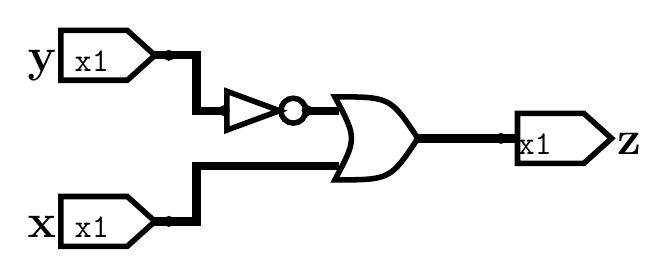
\begin{tikzpicture}[x=1pt,y=-1pt,line cap=rect]
\def\logisimfontA#1{\fontfamily{cmr}{#1}} % Replaced by logisim, original font was "SansSerif"
\def\logisimfontB#1{\fontfamily{cmtt}{#1}} % Replaced by logisim, original font was "Monospaced"
\definecolor{custcol_0_0_0}{RGB}{0, 0, 0}
\definecolor{custcol_ff_ff_ff}{RGB}{255, 255, 255}
\draw [line width=3.0pt, custcol_0_0_0 ]  (146.0,45.0) -- (176.0,45.0) ;
\draw [line width=3.0pt, custcol_0_0_0 ]  (106.0,35.0) -- (116.0,35.0) -- (116.0,35.0) ;
\draw [line width=2.0pt, custcol_0_0_0 ]  (146.0,45.0) .. controls  (136.0,30.0)  ..  (116.0,30.0) .. controls  (124.0,45.0)  ..  (116.0,60.0) .. controls  (136.0,60.0)  ..  (146.0,45.0) -- cycle ;
\draw [line width=2.0pt, custcol_0_0_0 ]  (96.0,35.0) -- (77.0,28.0) -- (77.0,42.0) -- cycle;
\draw [line width=2.0pt, custcol_0_0_0]  (101.0,35.0) ellipse (4.5 and 4.5 );
\fill [line width=2.0pt, custcol_0_0_0]  (106.0,35.0) ellipse (2.0 and 2.0 );
\fill [line width=2.0pt, custcol_0_0_0]  (76.0,35.0) ellipse (2.0 and 2.0 );
\draw [line width=3.0pt, custcol_0_0_0 ]  (180.0,45.0) -- (177.0,45.0) ;
\draw [line width=2.0pt, custcol_0_0_0 ]  (206.0,36.0) -- (216.0,45.0) -- (206.0,54.0) -- (182.0,54.0) -- (182.0,36.0) -- cycle;
\logisimfontB{\fontsize{12pt}{12pt}\selectfont\node[inner sep=0, outer sep=0, custcol_0_0_0, anchor=base west] at  (182.0,51.0)  {x1};}
\logisimfontA{\fontsize{16pt}{16pt}\fontseries{bx}\selectfont\node[inner sep=0, outer sep=0, custcol_0_0_0, anchor=base west] at  (218.0,51.0)  {z};}
\fill [line width=2.0pt, custcol_0_0_0]  (176.0,45.0) ellipse (2.0 and 2.0 );
\draw [line width=3.0pt, custcol_0_0_0 ]  (51.0,75.0) -- (56.0,75.0) -- (66.0,75.0) -- (66.0,55.0) -- (116.0,55.0) -- (116.0,55.0) ;
\draw [line width=2.0pt, custcol_0_0_0 ]  (41.0,84.0) -- (51.0,75.0) -- (41.0,66.0) -- (17.0,66.0) -- (17.0,84.0) -- cycle;
\logisimfontB{\fontsize{12pt}{12pt}\selectfont\node[inner sep=0, outer sep=0, custcol_0_0_0, anchor=base west] at  (22.0,81.0)  {x1};}
\logisimfontA{\fontsize{16pt}{16pt}\fontseries{bx}\selectfont\node[inner sep=0, outer sep=0, custcol_0_0_0, anchor=base west] at  (5.0,81.0)  {x};}
\fill [line width=2.0pt, custcol_0_0_0]  (56.0,75.0) ellipse (2.0 and 2.0 );
\draw [line width=3.0pt, custcol_0_0_0 ]  (51.0,15.0) -- (56.0,15.0) -- (66.0,15.0) -- (66.0,35.0) -- (76.0,35.0) ;
\draw [line width=2.0pt, custcol_0_0_0 ]  (41.0,24.0) -- (51.0,15.0) -- (41.0,6.0) -- (17.0,6.0) -- (17.0,24.0) -- cycle;
\logisimfontB{\fontsize{12pt}{12pt}\selectfont\node[inner sep=0, outer sep=0, custcol_0_0_0, anchor=base west] at  (22.0,21.0)  {x1};}
\logisimfontA{\fontsize{16pt}{16pt}\fontseries{bx}\selectfont\node[inner sep=0, outer sep=0, custcol_0_0_0, anchor=base west] at  (5.0,21.0)  {y};}
\fill [line width=2.0pt, custcol_0_0_0]  (56.0,15.0) ellipse (2.0 and 2.0 );
\end{tikzpicture}
}

			\label{fig:exe09}
		\end{figure}
	\end{columns}
\end{frame}

\section{Mintermos e Maxtermos}

\begin{frame}
	\frametitle{Mintermos e Maxtermos}
	\framesubtitle{Introdução}
	\par Até agora, determinamos as expressões algébricas de forma intuitiva, analisando os circuitos e os resultados das tabelas verdade para, geralmente, identificar a expressão lógica correspondente ao circuito. A partir de agora, utilizaremos ferramentas que oferece um método bem definido para montar a expressão algébrica correspondente ao circuito analisado.
	\par Tais ferramentas se chamam \textit{Mintermos} e \textit{Maxtermos} que, embora não produzam uma expressão otimizada, fornecem uma função inicial que pode ser manipulada e minimizada se assim o desejarmos.
\end{frame}

\begin{frame}
	\frametitle{Mintermos e Maxtermos}
	\framesubtitle{Definição}
	\begin{itemize}
		\item \textbf{Mintermos (Soma de Produtos Canônica (SOP)):} A função é expressa como a soma (OR) das linhas onde a função vale 1.
		\item \textbf{Maxtermos (Produto de Somas Canônica (POS)):} A função é expressa como o produto (AND) das linhas onde a função vale 0.
	\end{itemize}
\end{frame}

\begin{frame}
	\frametitle{Mintermos e Maxtermos}
	\framesubtitle{Definição e propriedades da soma de produtos canônica (SOP)}
	\begin{itemize}
		\item A implementação canônica de uma função booleana que seleciona os produtos das variáveis onde o resultado é 1.
		\item Propriedades:
		\begin{itemize}
			\item Unicidade: Existe uma única SOP canônica para cada função booleana.
			\item Importância: Útil na análise e síntese de circuitos digitais.
			\item Minimização: Pode ser simplificada com Mapas de Karnaugh ou Quine-McCluskey.
		\end{itemize}
	\end{itemize}
\end{frame}

\begin{frame}
	\frametitle{Mintermos e Maxtermos}
	\framesubtitle{Definição e Propriedades do produto de somas canônica (POS)}
	\begin{itemize}
		\item Forma canônica que seleciona as somas das variáveis onde o resultado é 0.
		\item Propriedades:
		\begin{itemize}
			\item Unicidade: Existe uma única POS canônica para cada função booleana.
			\item Importância: Utilizada em design digital para implementar lógica com portas OR e AND.
			\item Minimização: Pode ser simplificada como a SOP canônica.
		\end{itemize}
	\end{itemize}
\end{frame}


\begin{frame}
	\frametitle{Mintermos e Maxtermos}
	\framesubtitle{Exemplo de determinação de função lógica}
	
	\par Vamos determinar a \textbf{função lógica} a partir da tabela verdade abaixo:
	
	\[
	\begin{array}{|c|c|c|c|}
		\hline
		\textbf{a} & \textbf{b} & \textbf{c} & \textbf{f(a, b, c)} \\
		\hline
		0 & 0 & 0 & 0 \\
		0 & 0 & 1 & 1 \\
		0 & 1 & 0 & 0 \\
		0 & 1 & 1 & 1 \\
		1 & 0 & 0 & 1 \\
		1 & 0 & 1 & 1 \\
		1 & 1 & 0 & 0 \\
		1 & 1 & 1 & 0 \\
		\hline
	\end{array}
	\]
\end{frame}

\begin{frame}
	\frametitle{Mintermos e Maxtermos}
	\framesubtitle{Determinação da função lógica usando Mintermos}
	\begin{columns}
		\column{.35\linewidth}
			\par \textcolor{blue}{Mintermos}: Linhas onde $f(a, b, c) = 1$. \\ \textcolor{green}{Maxtermos} Linhas onde $f(a, b, c) = 0$.
			\[
			\begin{array}{|c|c|c|c|}
				\hline
				\textbf{a} & \textbf{b} & \textbf{c} & \textbf{f(a, b, c)} \\
				\hline
				0 & 0 & 0 & \cellcolor{green} 0 \\
				0 & 0 & 1 & \cellcolor{blue} 1 \\
				0 & 1 & 0 & \cellcolor{green} 0 \\
				0 & 1 & 1 & \cellcolor{blue} 1 \\
				1 & 0 & 0 & \cellcolor{blue} 1 \\
				1 & 0 & 1 & \cellcolor{blue} 1 \\
				1 & 1 & 0 & \cellcolor{green} 0 \\
				1 & 1 & 1 & \cellcolor{green} 0 \\
				\hline
			\end{array}
			\]
		\column{.65\linewidth}
			\par \textbf{Passo 1:} Identifique as linhas onde \(f(a, b, c) = 1\).
			\begin{itemize}
				\item 02: \(a = 0\), \(b = 0\), \(c = 1\)  \(\rightarrow\) Mintermo: \(\overline{a}.\overline{b}.c\)
				\item 04: \(a = 0\), \(b = 1\), \(c = 1\)  \(\rightarrow\) Mintermo: \(\overline{a}.bc\)
				\item 05: \(a = 1\), \(b = 0\), \(c = 0\)  \(\rightarrow\) Mintermo: \(a\overline{b}.\overline{c}\)
				\item 06: \(a = 1\), \(b = 0\), \(c = 1\)  \(\rightarrow\) Mintermo: \(a\overline{b}.c\)
			\end{itemize}
			
			\par \textbf{Passo 2:} Escreva a função como a soma (OR) desses mintermos.\newline
			
			\par A função lógica pode ser expressa como a soma dos mintermos correspondentes: \\$\boxed{f(a, b, c) = \overline{a}.\overline{b}.c + \overline{a}bc + a\overline{b}\overline{c} + ab\overline{c}}$
	\end{columns}
	
\end{frame}

\begin{frame}
	\frametitle{Mintermos e Maxtermos}
	\framesubtitle{Determinação da função lógica usando Maxtermos}
	\begin{columns}
		\column{.35\linewidth}
			\par \textcolor{blue}{Mintermos}: Linhas onde $f(a, b, c) = 1$. \\ \textcolor{green}{Maxtermos} Linhas onde $f(a, b, c) = 0$.
			\[
			\begin{array}{|c|c|c|c|}
				\hline
				\textbf{a} & \textbf{b} & \textbf{c} & \textbf{f(a, b, c)} \\
				\hline
				0 & 0 & 0 & \cellcolor{green} 0 \\
				0 & 0 & 1 & \cellcolor{blue} 1 \\
				0 & 1 & 0 & \cellcolor{green} 0 \\
				0 & 1 & 1 & \cellcolor{blue} 1 \\
				1 & 0 & 0 & \cellcolor{blue} 1 \\
				1 & 0 & 1 & \cellcolor{blue} 1 \\
				1 & 1 & 0 & \cellcolor{green} 0 \\
				1 & 1 & 1 & \cellcolor{green} 0 \\
				\hline
			\end{array}
			\]
		\column{.65\linewidth}
			\par \textbf{Passo 1:} Identifique as linhas onde \(f(a, b, c) = 0\).
			\begin{itemize}
				\item 01: \(a = 0\), \(b = 0\), \(c = 0\)  \(\rightarrow\) Maxtermo: \(a + b + c\)
				\item 03: \(a = 0\), \(b = 1\), \(c = 0\)  \(\rightarrow\) Maxtermo: \(a + \overline{b} + c\)
				\item 07: \(a = 1\), \(b = 1\), \(c = 0\)  \(\rightarrow\) Maxtermo: \(\overline{a} + b + c\)
				\item 08: \(a = 1\), \(b = 1\), \(c = 1\)  \(\rightarrow\) Maxtermo: \(\overline{a} + b + \overline{c}\)
			\end{itemize}
			
			\textbf{Passo 2:} Escreva a função como o produto (AND) desses maxtermos.\newline
			
			A função lógica pode ser expressa como o produto dos maxtermos correspondentes:$f(a, b, c) =$ \\ $\boxed{(a + b + c) \cdot (a + \overline{b} + c) \cdot (\overline{a} + b + c) \cdot (\overline{a} + b + \overline{c})}$
		\end{columns}
\end{frame}


\begin{frame}{SOP - Prática guiada 01}
	\begin{itemize}
		\item Considere a função f(a, b, c) definida pela tabela verdade:
		\item \textbf{tabela verdade:}
		\begin{tabular}{|c|c|c|c|}
			\hline
			a & b & c & f(a, b, c) \\
			\hline
			0 & 0 & 0 & 0 \\
			0 & 0 & 1 & 1 \\
			0 & 1 & 0 & 0 \\
			0 & 1 & 1 & 1 \\
			1 & 0 & 0 & 1 \\
			1 & 0 & 1 & 1 \\
			1 & 1 & 0 & 0 \\
			1 & 1 & 1 & 1 \\
			\hline
		\end{tabular}
		\item \textbf{Mintermos:}
		\begin{itemize}
			\item $\overline{a}\overline{b}c, \overline{a}bc, a\overline{b}\overline{c}, ab\overline{c}, abc$
		\end{itemize}
		\item \textbf{SOP Canônica:}
		$f(a,b,c) = \overline{a}\overline{b}c + \overline{a}bc + a\overline{b}\overline{c} + ab\overline{c} + abc$
	\end{itemize}
\end{frame}

\begin{frame}{POS - Prática guiada 02}
	\begin{itemize}
		\item Considere a função f(a, b, c) definida pela tabela verdade:
		\item \textbf{tabela verdade:}
		\begin{tabular}{|c|c|c|c|}
			\hline
			a & b & c & f(a, b, c) \\
			\hline
			0 & 0 & 0 & 0 \\
			0 & 0 & 1 & 1 \\
			0 & 1 & 0 & 0 \\
			0 & 1 & 1 & 1 \\
			1 & 0 & 0 & 1 \\
			1 & 0 & 1 & 1 \\
			1 & 1 & 0 & 0 \\
			1 & 1 & 1 & 1 \\
			\hline
		\end{tabular}
		\item \textbf{Maxtermos:}
		\begin{itemize}
			\item $(a + b + c), (a + \overline{b} + c), (\overline{a} + b + \overline{c})$
		\end{itemize}
		\item \textbf{POS Canônica:}
		$f(a,b,c) = (a + b + c) \cdot (a + \overline{b} + c) \cdot (\overline{a} + b + \overline{c})$
	\end{itemize}
\end{frame}

\begin{frame}{Exercício}
	\par Criação de Circuito a partir da tabela verdade
	\begin{itemize}
		\item Dada a seguinte tabela verdade:
		\[
		\begin{array}{|c|c|c|c|}
			\hline
			x & y & z & f(x, y, z) \\
			\hline
			0 & 0 & 0 & 0 \\
			0 & 0 & 1 & 1 \\
			0 & 1 & 0 & 0 \\
			0 & 1 & 1 & 1 \\
			1 & 0 & 0 & 1 \\
			1 & 0 & 1 & 0 \\
			1 & 1 & 0 & 0 \\
			1 & 1 & 1 & 1 \\
			\hline
		\end{array}
		\]
		\begin{enumerate}
			\item Construa o circuito digital que implementa essa função.
			\item Derive a expressão algébrica na forma de Soma de Produtos Canônica (SOP) a partir da tabela verdade.
			\item Crie o diagrama de tempo correspondente ao circuito.
		\end{enumerate}
	\end{itemize}
\end{frame}

\begin{frame}{Exercício - Resolução}
	
	\begin{columns}
		\column{.5\linewidth}
			\par Selecionando os \textcolor{green}{mintermos} (Soma de Produtos Canônica)
			\[\begin{array}{|c|c|c|c|}
				\hline
				x & y & z & f(x, y, z) \\
				\hline
				0 & 0 & 0 & 0 \\
				0 & 0 & 1 & \cellcolor{green} 1 \\
				0 & 1 & 0 & 0 \\
				0 & 1 & 1 & \cellcolor{green} 1 \\
				1 & 0 & 0 & \cellcolor{green} 1 \\
				1 & 0 & 1 & 0 \\
				1 & 1 & 0 & 0 \\
				1 & 1 & 1 & \cellcolor{green} 1 \\
				\hline
			\end{array}\]
			\par $f(x,y,z) = (\overline{x}\overline{y}z)+(\overline{x}yz)+(x\overline{y}\overline{z})+(xyz)$
		\column{.5\linewidth}
			\par Agrupando $(\overline{x}yz)+(xyz) = (yz).(\overline{x}+x) = (yz) . 1 = \boxed{yz}$
			\par Agrupando $yz$ com o restante da expressão $\boxed{yz}+(\overline{x}\overline{y}z)+(x\overline{y}\overline{z})$.\newline
			\par Fatorando $z$: $z.(y + \overline{x}\overline{y})+(x\overline{y}\overline{z}) = z.(\overline{x}+y)+(x\overline{y}\overline{z}) = \boxed{\overline{x}z+yz+x\overline{y}\overline{z}}$
			\begin{figure}
				\centering
				% Important: If latex complains about unicode characters,
% please use "\usepackage[utf8x]{inputenc}" in your preamble
% You can change the size of the picture by putting it into the construct:
% 1) \resizebox{10cm}{!}{"below picture"} to scale horizontally to 10 cm
% 2) \resizebox{!}{15cm}{"below picture"} to scale vertically to 15 cm
% 3) \resizebox{10cm}{15cm}{"below picture"} a combination of above two
% It is not recomended to use the scale option of the tikzpicture environment.
\resizebox{7cm}{!}{
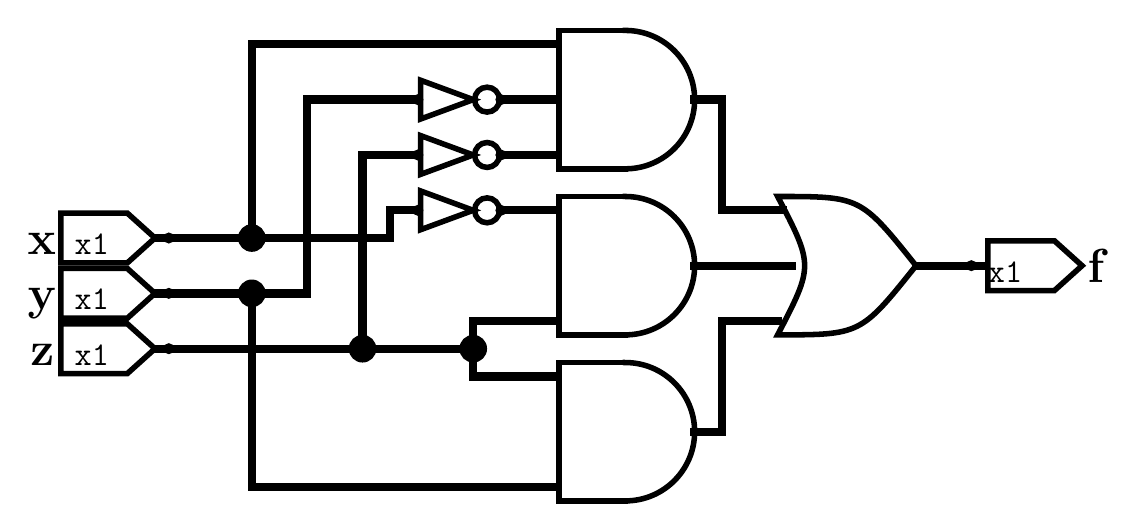
\begin{tikzpicture}[x=1pt,y=-1pt,line cap=rect]
\def\logisimfontA#1{\fontfamily{cmr}{#1}} % Replaced by logisim, original font was "SansSerif"
\def\logisimfontB#1{\fontfamily{cmtt}{#1}} % Replaced by logisim, original font was "Monospaced"
\definecolor{custcol_0_0_0}{RGB}{0, 0, 0}
\definecolor{custcol_ff_ff_ff}{RGB}{255, 255, 255}
\draw [line width=3.0pt, custcol_0_0_0 ]  (326.0,90.0) -- (346.0,90.0) ;
\draw [line width=3.0pt, custcol_0_0_0 ]  (196.0,10.0) -- (86.0,10.0) -- (86.0,80.0) -- (136.0,80.0) -- (136.0,70.0) -- (146.0,70.0) ;
\draw [line width=3.0pt, custcol_0_0_0 ]  (126.0,120.0) -- (166.0,120.0) ;
\draw [line width=3.0pt, custcol_0_0_0 ]  (196.0,110.0) -- (166.0,110.0) -- (166.0,120.0) -- (166.0,130.0) -- (196.0,130.0) ;
\draw [line width=3.0pt, custcol_0_0_0 ]  (176.0,50.0) -- (196.0,50.0) ;
\draw [line width=3.0pt, custcol_0_0_0 ]  (176.0,30.0) -- (196.0,30.0) ;
\draw [line width=3.0pt, custcol_0_0_0 ]  (176.0,70.0) -- (196.0,70.0) ;
\draw [line width=3.0pt, custcol_0_0_0 ]  (86.0,100.0) -- (106.0,100.0) -- (106.0,30.0) -- (146.0,30.0) ;
\fill [line width=3.0pt, custcol_0_0_0]  (166.0,120.0) ellipse (5.0 and 5.0 );
\fill [line width=3.0pt, custcol_0_0_0]  (126.0,120.0) ellipse (5.0 and 5.0 );
\fill [line width=3.0pt, custcol_0_0_0]  (86.0,80.0) ellipse (5.0 and 5.0 );
\fill [line width=3.0pt, custcol_0_0_0]  (86.0,100.0) ellipse (5.0 and 5.0 );
\draw [line width=3.0pt, custcol_0_0_0 ]  (350.0,90.0) -- (347.0,90.0) ;
\draw [line width=2.0pt, custcol_0_0_0 ]  (376.0,81.0) -- (386.0,90.0) -- (376.0,99.0) -- (352.0,99.0) -- (352.0,81.0) -- cycle;
\logisimfontB{\fontsize{12pt}{12pt}\selectfont\node[inner sep=0, outer sep=0, custcol_0_0_0, anchor=base west] at  (352.0,96.0)  {x1};}
\logisimfontA{\fontsize{16pt}{16pt}\fontseries{bx}\selectfont\node[inner sep=0, outer sep=0, custcol_0_0_0, anchor=base west] at  (388.0,96.0)  {f};}
\fill [line width=2.0pt, custcol_0_0_0]  (346.0,90.0) ellipse (2.0 and 2.0 );
\draw [line width=3.0pt, custcol_0_0_0 ]  (51.0,120.0) -- (56.0,120.0) -- (126.0,120.0) -- (126.0,50.0) -- (146.0,50.0) ;
\draw [line width=2.0pt, custcol_0_0_0 ]  (41.0,129.0) -- (51.0,120.0) -- (41.0,111.0) -- (17.0,111.0) -- (17.0,129.0) -- cycle;
\logisimfontB{\fontsize{12pt}{12pt}\selectfont\node[inner sep=0, outer sep=0, custcol_0_0_0, anchor=base west] at  (22.0,126.0)  {x1};}
\logisimfontA{\fontsize{16pt}{16pt}\fontseries{bx}\selectfont\node[inner sep=0, outer sep=0, custcol_0_0_0, anchor=base west] at  (6.0,126.0)  {z};}
\fill [line width=2.0pt, custcol_0_0_0]  (56.0,120.0) ellipse (2.0 and 2.0 );
\draw [line width=3.0pt, custcol_0_0_0 ]  (51.0,100.0) -- (56.0,100.0) -- (86.0,100.0) -- (86.0,170.0) -- (196.0,170.0) ;
\draw [line width=2.0pt, custcol_0_0_0 ]  (41.0,109.0) -- (51.0,100.0) -- (41.0,91.0) -- (17.0,91.0) -- (17.0,109.0) -- cycle;
\logisimfontB{\fontsize{12pt}{12pt}\selectfont\node[inner sep=0, outer sep=0, custcol_0_0_0, anchor=base west] at  (22.0,106.0)  {x1};}
\logisimfontA{\fontsize{16pt}{16pt}\fontseries{bx}\selectfont\node[inner sep=0, outer sep=0, custcol_0_0_0, anchor=base west] at  (5.0,106.0)  {y};}
\fill [line width=2.0pt, custcol_0_0_0]  (56.0,100.0) ellipse (2.0 and 2.0 );
\draw [line width=3.0pt, custcol_0_0_0 ]  (246.0,30.0) -- (256.0,30.0) -- (256.0,70.0) -- (276.0,70.0) -- (278.0,70.0) ;
\draw [line width=3.0pt, custcol_0_0_0 ]  (246.0,90.0) -- (276.0,90.0) -- (281.0,90.0) ;
\draw [line width=3.0pt, custcol_0_0_0 ]  (246.0,150.0) -- (256.0,150.0) -- (256.0,110.0) -- (276.0,110.0) -- (276.0,110.0) ;
\draw [line width=2.0pt, custcol_0_0_0 ]  (326.0,90.0) .. controls  (306.0,65.0)  ..  (276.0,65.0) .. controls  (289.0,90.0)  ..  (276.0,115.0) .. controls  (306.0,115.0)  ..  (326.0,90.0) -- cycle ;
\draw [line width=2.0pt, custcol_0_0_0 ]  (166.0,70.0) -- (147.0,63.0) -- (147.0,77.0) -- cycle;
\draw [line width=2.0pt, custcol_0_0_0]  (171.0,70.0) ellipse (4.5 and 4.5 );
\fill [line width=2.0pt, custcol_0_0_0]  (176.0,70.0) ellipse (2.0 and 2.0 );
\fill [line width=2.0pt, custcol_0_0_0]  (146.0,70.0) ellipse (2.0 and 2.0 );
\draw [line width=2.0pt, custcol_0_0_0] (221.0,115.0) arc (90.0:-90.0:25.0 and 25.0 );
\draw [line width=2.0pt, custcol_0_0_0 ]  (221.0,65.0) -- (197.0,65.0) -- (197.0,115.0) -- (221.0,115.0) ;
\draw [line width=2.0pt, custcol_0_0_0 ]  (166.0,30.0) -- (147.0,23.0) -- (147.0,37.0) -- cycle;
\draw [line width=2.0pt, custcol_0_0_0]  (171.0,30.0) ellipse (4.5 and 4.5 );
\fill [line width=2.0pt, custcol_0_0_0]  (176.0,30.0) ellipse (2.0 and 2.0 );
\fill [line width=2.0pt, custcol_0_0_0]  (146.0,30.0) ellipse (2.0 and 2.0 );
\draw [line width=2.0pt, custcol_0_0_0 ]  (166.0,50.0) -- (147.0,43.0) -- (147.0,57.0) -- cycle;
\draw [line width=2.0pt, custcol_0_0_0]  (171.0,50.0) ellipse (4.5 and 4.5 );
\fill [line width=2.0pt, custcol_0_0_0]  (176.0,50.0) ellipse (2.0 and 2.0 );
\fill [line width=2.0pt, custcol_0_0_0]  (146.0,50.0) ellipse (2.0 and 2.0 );
\draw [line width=3.0pt, custcol_0_0_0 ]  (51.0,80.0) -- (56.0,80.0) -- (86.0,80.0) ;
\draw [line width=2.0pt, custcol_0_0_0 ]  (41.0,89.0) -- (51.0,80.0) -- (41.0,71.0) -- (17.0,71.0) -- (17.0,89.0) -- cycle;
\logisimfontB{\fontsize{12pt}{12pt}\selectfont\node[inner sep=0, outer sep=0, custcol_0_0_0, anchor=base west] at  (22.0,86.0)  {x1};}
\logisimfontA{\fontsize{16pt}{16pt}\fontseries{bx}\selectfont\node[inner sep=0, outer sep=0, custcol_0_0_0, anchor=base west] at  (5.0,86.0)  {x};}
\fill [line width=2.0pt, custcol_0_0_0]  (56.0,80.0) ellipse (2.0 and 2.0 );
\draw [line width=2.0pt, custcol_0_0_0] (221.0,175.0) arc (90.0:-90.0:25.0 and 25.0 );
\draw [line width=2.0pt, custcol_0_0_0 ]  (221.0,125.0) -- (197.0,125.0) -- (197.0,175.0) -- (221.0,175.0) ;
\draw [line width=2.0pt, custcol_0_0_0] (221.0,55.0) arc (90.0:-90.0:25.0 and 25.0 );
\draw [line width=2.0pt, custcol_0_0_0 ]  (221.0,5.0) -- (197.0,5.0) -- (197.0,55.0) -- (221.0,55.0) ;
\end{tikzpicture}
}


				\label{fig:exe15}
			\end{figure}
			
	\end{columns}
\end{frame}

\begin{frame}{Mini prova 03}
	\begin{itemize}
		\item Dado o circuito abaixo, determine:
		\begin{enumerate}
			\item A tabela verdade correspondente ao circuito \textbf{não simplificado}.
			\item A expressão algébrica \textbf{simplificada} que representa a função lógica do circuito.
			\item O circuito simplificado.
			\item O diagrama de tempo (waveform) que reflete o comportamento do circuito.
		\end{enumerate}
	\end{itemize}
	\begin{figure}
		\centering
		% Important: If latex complains about unicode characters,
% please use "\usepackage[utf8x]{inputenc}" in your preamble
% You can change the size of the picture by putting it into the construct:
% 1) \resizebox{10cm}{!}{"below picture"} to scale horizontally to 10 cm
% 2) \resizebox{!}{15cm}{"below picture"} to scale vertically to 15 cm
% 3) \resizebox{10cm}{15cm}{"below picture"} a combination of above two
% It is not recomended to use the scale option of the tikzpicture environment.
\resizebox{10cm}{!}{
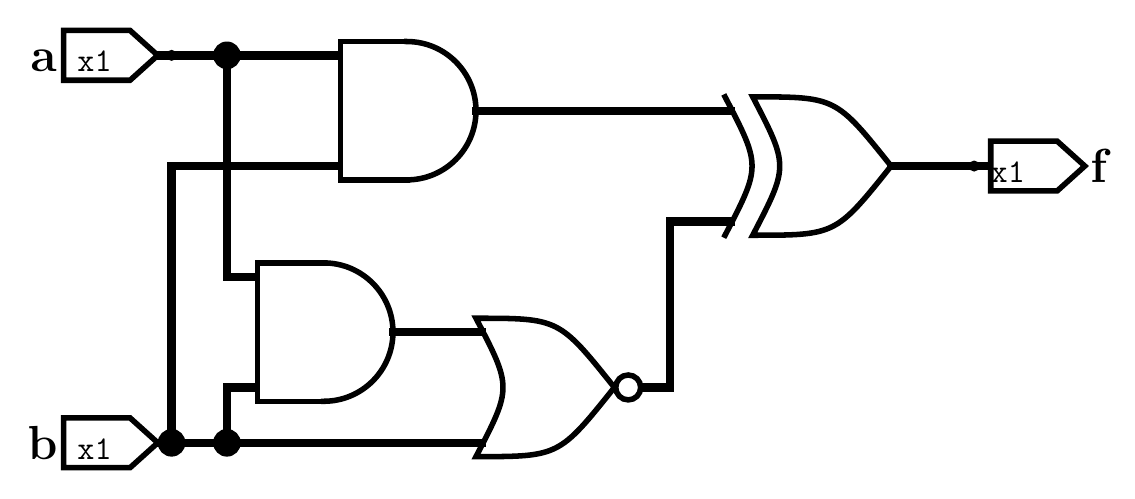
\begin{tikzpicture}[x=1pt,y=-1pt,line cap=rect]
\def\logisimfontA#1{\fontfamily{cmr}{#1}} % Replaced by logisim, original font was "SansSerif"
\def\logisimfontB#1{\fontfamily{cmtt}{#1}} % Replaced by logisim, original font was "Monospaced"
\definecolor{custcol_0_0_0}{RGB}{0, 0, 0}
\definecolor{custcol_ff_ff_ff}{RGB}{255, 255, 255}
\draw [line width=3.0pt, custcol_0_0_0 ]  (317.0,55.0) -- (347.0,55.0) ;
\draw [line width=3.0pt, custcol_0_0_0 ]  (117.0,55.0) -- (57.0,55.0) -- (57.0,155.0) -- (77.0,155.0) ;
\draw [line width=3.0pt, custcol_0_0_0 ]  (117.0,15.0) -- (77.0,15.0) -- (77.0,95.0) -- (87.0,95.0) ;
\fill [line width=3.0pt, custcol_0_0_0]  (57.0,155.0) ellipse (5.0 and 5.0 );
\fill [line width=3.0pt, custcol_0_0_0]  (77.0,15.0) ellipse (5.0 and 5.0 );
\fill [line width=3.0pt, custcol_0_0_0]  (77.0,155.0) ellipse (5.0 and 5.0 );
\draw [line width=3.0pt, custcol_0_0_0 ]  (52.0,155.0) -- (57.0,155.0) ;
\draw [line width=2.0pt, custcol_0_0_0 ]  (42.0,164.0) -- (52.0,155.0) -- (42.0,146.0) -- (18.0,146.0) -- (18.0,164.0) -- cycle;
\logisimfontB{\fontsize{12pt}{12pt}\selectfont\node[inner sep=0, outer sep=0, custcol_0_0_0, anchor=base west] at  (23.0,161.0)  {x1};}
\logisimfontA{\fontsize{16pt}{16pt}\fontseries{bx}\selectfont\node[inner sep=0, outer sep=0, custcol_0_0_0, anchor=base west] at  (5.0,161.0)  {b};}
\fill [line width=2.0pt, custcol_0_0_0]  (57.0,155.0) ellipse (2.0 and 2.0 );
\draw [line width=3.0pt, custcol_0_0_0 ]  (137.0,115.0) -- (167.0,115.0) -- (169.0,115.0) ;
\draw [line width=3.0pt, custcol_0_0_0 ]  (87.0,135.0) -- (77.0,135.0) -- (77.0,155.0) -- (167.0,155.0) -- (169.0,155.0) ;
\draw [line width=2.0pt, custcol_0_0_0 ]  (217.0,135.0) .. controls  (197.0,110.0)  ..  (167.0,110.0) .. controls  (180.0,135.0)  ..  (167.0,160.0) .. controls  (197.0,160.0)  ..  (217.0,135.0) -- cycle ;
\draw [line width=2.0pt, custcol_0_0_0]  (222.0,135.0) ellipse (4.5 and 4.5 );
\draw [line width=2.0pt, custcol_0_0_0] (112.0,140.0) arc (90.0:-90.0:25.0 and 25.0 );
\draw [line width=2.0pt, custcol_0_0_0 ]  (112.0,90.0) -- (88.0,90.0) -- (88.0,140.0) -- (112.0,140.0) ;
\draw [line width=3.0pt, custcol_0_0_0 ]  (52.0,15.0) -- (57.0,15.0) -- (77.0,15.0) ;
\draw [line width=2.0pt, custcol_0_0_0 ]  (42.0,24.0) -- (52.0,15.0) -- (42.0,6.0) -- (18.0,6.0) -- (18.0,24.0) -- cycle;
\logisimfontB{\fontsize{12pt}{12pt}\selectfont\node[inner sep=0, outer sep=0, custcol_0_0_0, anchor=base west] at  (23.0,21.0)  {x1};}
\logisimfontA{\fontsize{16pt}{16pt}\fontseries{bx}\selectfont\node[inner sep=0, outer sep=0, custcol_0_0_0, anchor=base west] at  (6.0,21.0)  {a};}
\fill [line width=2.0pt, custcol_0_0_0]  (57.0,15.0) ellipse (2.0 and 2.0 );
\draw [line width=3.0pt, custcol_0_0_0 ]  (167.0,35.0) -- (257.0,35.0) -- (259.0,35.0) ;
\draw [line width=3.0pt, custcol_0_0_0 ]  (227.0,135.0) -- (237.0,135.0) -- (237.0,75.0) -- (257.0,75.0) -- (259.0,75.0) ;
\draw [line width=2.0pt, custcol_0_0_0 ]  (317.0,55.0) .. controls  (297.0,30.0)  ..  (267.0,30.0) .. controls  (280.0,55.0)  ..  (267.0,80.0) .. controls  (297.0,80.0)  ..  (317.0,55.0) -- cycle ;
\draw [line width=2.0pt, custcol_0_0_0 ]  (257.0,30.0) .. controls  (270.0,55.0)  ..  (257.0,80.0) ;
\draw [line width=3.0pt, custcol_0_0_0 ]  (351.0,55.0) -- (348.0,55.0) ;
\draw [line width=2.0pt, custcol_0_0_0 ]  (377.0,46.0) -- (387.0,55.0) -- (377.0,64.0) -- (353.0,64.0) -- (353.0,46.0) -- cycle;
\logisimfontB{\fontsize{12pt}{12pt}\selectfont\node[inner sep=0, outer sep=0, custcol_0_0_0, anchor=base west] at  (353.0,61.0)  {x1};}
\logisimfontA{\fontsize{16pt}{16pt}\fontseries{bx}\selectfont\node[inner sep=0, outer sep=0, custcol_0_0_0, anchor=base west] at  (389.0,61.0)  {f};}
\fill [line width=2.0pt, custcol_0_0_0]  (347.0,55.0) ellipse (2.0 and 2.0 );
\draw [line width=2.0pt, custcol_0_0_0] (142.0,60.0) arc (90.0:-90.0:25.0 and 25.0 );
\draw [line width=2.0pt, custcol_0_0_0 ]  (142.0,10.0) -- (118.0,10.0) -- (118.0,60.0) -- (142.0,60.0) ;
\end{tikzpicture}
}

		\caption{Passarinho... Resolve esse... Qual é a expressão desse?\footnote[frame]{\textit{referência de velho}}}
		\label{fig:05exe}
	\end{figure}
\end{frame}

\section{\musEighth All you need is NAND/NOR... \musEighth}

\begin{frame}
	\frametitle{O que fazer se você não tem as portas lógicas que vc precisa}
	\par $\overline{a} = a\downarrow a = a \uparrow a$
	\begin{figure}
		\centering
		% Important: If latex complains about unicode characters,
% please use "\usepackage[utf8x]{inputenc}" in your preamble
% You can change the size of the picture by putting it into the construct:
% 1) \resizebox{10cm}{!}{"below picture"} to scale horizontally to 10 cm
% 2) \resizebox{!}{15cm}{"below picture"} to scale vertically to 15 cm
% 3) \resizebox{10cm}{15cm}{"below picture"} a combination of above two
% It is not recomended to use the scale option of the tikzpicture environment.
\resizebox{10cm}{!}{
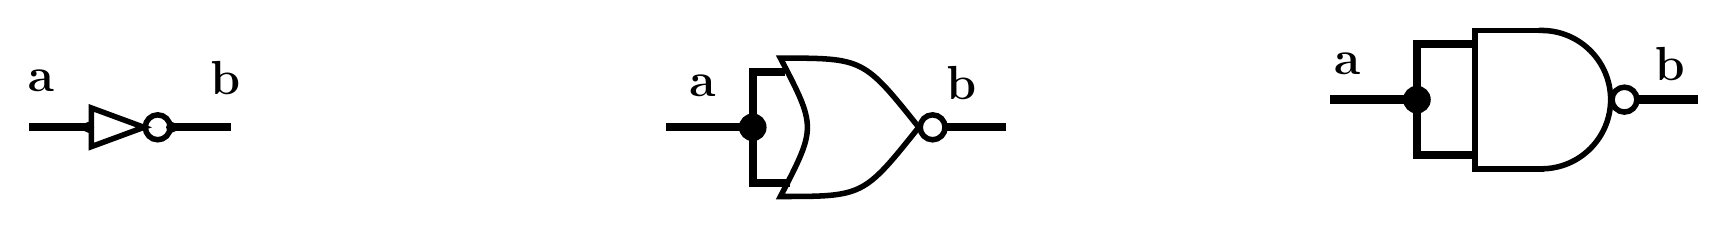
\begin{tikzpicture}[x=1pt,y=-1pt,line cap=rect]
\def\logisimfontA#1{\fontfamily{cmr}{#1}} % Replaced by logisim, original font was "SansSerif"
\definecolor{custcol_0_0_0}{RGB}{0, 0, 0}
\definecolor{custcol_ff_ff_ff}{RGB}{255, 255, 255}
\draw [line width=3.0pt, custcol_0_0_0 ]  (531.0,11.0) -- (511.0,11.0) -- (511.0,31.0) -- (511.0,51.0) -- (531.0,51.0) ;
\draw [line width=3.0pt, custcol_0_0_0 ]  (591.0,31.0) -- (611.0,31.0) ;
\draw [line width=3.0pt, custcol_0_0_0 ]  (241.0,41.0) -- (271.0,41.0) ;
\draw [line width=3.0pt, custcol_0_0_0 ]  (341.0,41.0) -- (361.0,41.0) ;
\draw [line width=3.0pt, custcol_0_0_0 ]  (481.0,31.0) -- (511.0,31.0) ;
\draw [line width=3.0pt, custcol_0_0_0 ]  (11.0,41.0) -- (31.0,41.0) ;
\draw [line width=3.0pt, custcol_0_0_0 ]  (61.0,41.0) -- (81.0,41.0) ;
\fill [line width=3.0pt, custcol_0_0_0]  (271.0,41.0) ellipse (5.0 and 5.0 );
\fill [line width=3.0pt, custcol_0_0_0]  (511.0,31.0) ellipse (5.0 and 5.0 );
\draw [line width=2.0pt, custcol_0_0_0 ]  (51.0,41.0) -- (32.0,34.0) -- (32.0,48.0) -- cycle;
\draw [line width=2.0pt, custcol_0_0_0]  (56.0,41.0) ellipse (4.5 and 4.5 );
\fill [line width=2.0pt, custcol_0_0_0]  (61.0,41.0) ellipse (2.0 and 2.0 );
\fill [line width=2.0pt, custcol_0_0_0]  (31.0,41.0) ellipse (2.0 and 2.0 );
\logisimfontA{\fontsize{16pt}{16pt}\fontseries{bx}\selectfont\node[inner sep=0, outer sep=0, custcol_0_0_0, anchor=base west] at  (75.0,29.0)  {b};}
\logisimfontA{\fontsize{16pt}{16pt}\fontseries{bx}\selectfont\node[inner sep=0, outer sep=0, custcol_0_0_0, anchor=base west] at  (597.0,24.0)  {b};}
\logisimfontA{\fontsize{16pt}{16pt}\fontseries{bx}\selectfont\node[inner sep=0, outer sep=0, custcol_0_0_0, anchor=base west] at  (341.0,31.0)  {b};}
\logisimfontA{\fontsize{16pt}{16pt}\fontseries{bx}\selectfont\node[inner sep=0, outer sep=0, custcol_0_0_0, anchor=base west] at  (248.0,30.0)  {a};}
\draw [line width=2.0pt, custcol_0_0_0] (556.0,56.0) arc (90.0:-90.0:25.0 and 25.0 );
\draw [line width=2.0pt, custcol_0_0_0 ]  (556.0,6.0) -- (532.0,6.0) -- (532.0,56.0) -- (556.0,56.0) ;
\draw [line width=2.0pt, custcol_0_0_0]  (586.0,31.0) ellipse (4.5 and 4.5 );
\logisimfontA{\fontsize{16pt}{16pt}\fontseries{bx}\selectfont\node[inner sep=0, outer sep=0, custcol_0_0_0, anchor=base west] at  (9.0,28.0)  {a};}
\logisimfontA{\fontsize{16pt}{16pt}\fontseries{bx}\selectfont\node[inner sep=0, outer sep=0, custcol_0_0_0, anchor=base west] at  (481.0,22.0)  {a};}
\draw [line width=3.0pt, custcol_0_0_0 ]  (281.0,21.0) -- (281.0,21.0) -- (271.0,21.0) -- (271.0,41.0) -- (271.0,61.0) -- (281.0,61.0) -- (283.0,61.0) ;
\draw [line width=2.0pt, custcol_0_0_0 ]  (331.0,41.0) .. controls  (311.0,16.0)  ..  (281.0,16.0) .. controls  (294.0,41.0)  ..  (281.0,66.0) .. controls  (311.0,66.0)  ..  (331.0,41.0) -- cycle ;
\draw [line width=2.0pt, custcol_0_0_0]  (336.0,41.0) ellipse (4.5 and 4.5 );
\end{tikzpicture}
}

		\label{fig:nandnot}
	\end{figure}
	
	\par $a.b = (a \downarrow a)\downarrow(b\downarrow b) = (a\uparrow b)\uparrow(a\uparrow b)$
	\begin{figure}
		\centering
		% Important: If latex complains about unicode characters,
% please use "\usepackage[utf8x]{inputenc}" in your preamble
% You can change the size of the picture by putting it into the construct:
% 1) \resizebox{10cm}{!}{"below picture"} to scale horizontally to 10 cm
% 2) \resizebox{!}{15cm}{"below picture"} to scale vertically to 15 cm
% 3) \resizebox{10cm}{15cm}{"below picture"} a combination of above two
% It is not recomended to use the scale option of the tikzpicture environment.
\resizebox{10cm}{!}{
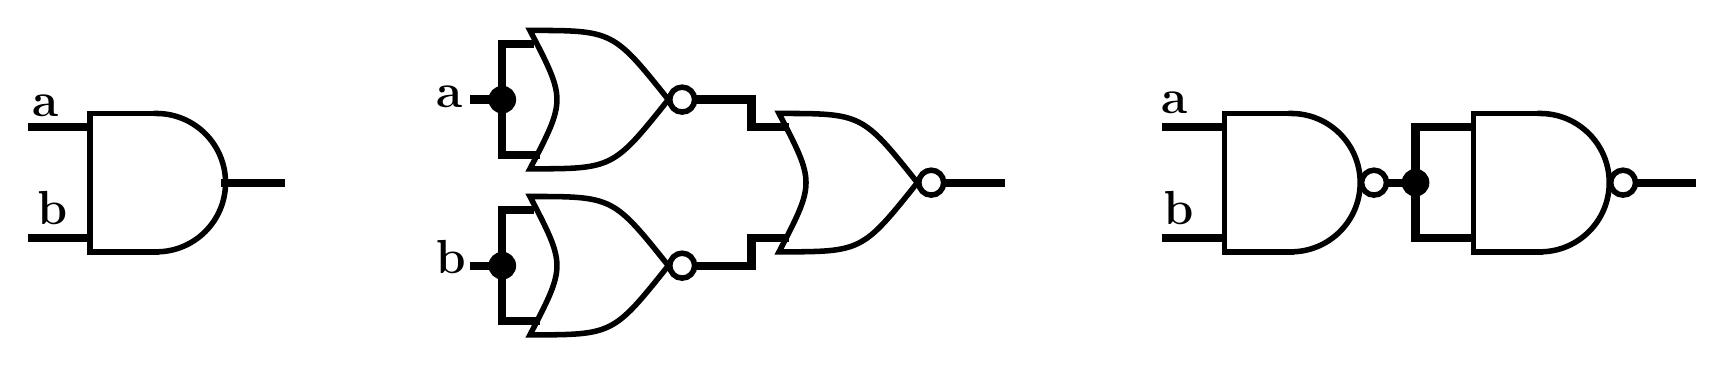
\begin{tikzpicture}[x=1pt,y=-1pt,line cap=rect]
\def\logisimfontA#1{\fontfamily{cmr}{#1}} % Replaced by logisim, original font was "SansSerif"
\definecolor{custcol_0_0_0}{RGB}{0, 0, 0}
\definecolor{custcol_ff_ff_ff}{RGB}{255, 255, 255}
\draw [line width=3.0pt, custcol_0_0_0 ]  (529.0,40.0) -- (509.0,40.0) -- (509.0,60.0) -- (509.0,80.0) -- (529.0,80.0) ;
\draw [line width=3.0pt, custcol_0_0_0 ]  (589.0,60.0) -- (609.0,60.0) ;
\draw [line width=3.0pt, custcol_0_0_0 ]  (339.0,60.0) -- (359.0,60.0) ;
\draw [line width=3.0pt, custcol_0_0_0 ]  (419.0,40.0) -- (439.0,40.0) ;
\draw [line width=3.0pt, custcol_0_0_0 ]  (419.0,80.0) -- (439.0,80.0) ;
\draw [line width=3.0pt, custcol_0_0_0 ]  (9.0,80.0) -- (29.0,80.0) ;
\draw [line width=3.0pt, custcol_0_0_0 ]  (9.0,40.0) -- (29.0,40.0) ;
\draw [line width=3.0pt, custcol_0_0_0 ]  (79.0,60.0) -- (99.0,60.0) ;
\draw [line width=3.0pt, custcol_0_0_0 ]  (169.0,90.0) -- (179.0,90.0) ;
\draw [line width=3.0pt, custcol_0_0_0 ]  (169.0,30.0) -- (179.0,30.0) ;
\draw [line width=3.0pt, custcol_0_0_0 ]  (499.0,60.0) -- (509.0,60.0) ;
\fill [line width=3.0pt, custcol_0_0_0]  (179.0,90.0) ellipse (5.0 and 5.0 );
\fill [line width=3.0pt, custcol_0_0_0]  (179.0,30.0) ellipse (5.0 and 5.0 );
\fill [line width=3.0pt, custcol_0_0_0]  (509.0,60.0) ellipse (5.0 and 5.0 );
\logisimfontA{\fontsize{16pt}{16pt}\fontseries{bx}\selectfont\node[inner sep=0, outer sep=0, custcol_0_0_0, anchor=base west] at  (155.0,93.0)  {b};}
\draw [line width=3.0pt, custcol_0_0_0 ]  (189.0,10.0) -- (189.0,10.0) -- (179.0,10.0) -- (179.0,30.0) -- (179.0,50.0) -- (189.0,50.0) -- (191.0,50.0) ;
\draw [line width=2.0pt, custcol_0_0_0 ]  (239.0,30.0) .. controls  (219.0,5.0)  ..  (189.0,5.0) .. controls  (202.0,30.0)  ..  (189.0,55.0) .. controls  (219.0,55.0)  ..  (239.0,30.0) -- cycle ;
\draw [line width=2.0pt, custcol_0_0_0]  (244.0,30.0) ellipse (4.5 and 4.5 );
\logisimfontA{\fontsize{16pt}{16pt}\fontseries{bx}\selectfont\node[inner sep=0, outer sep=0, custcol_0_0_0, anchor=base west] at  (418.0,75.0)  {b};}
\draw [line width=3.0pt, custcol_0_0_0 ]  (189.0,70.0) -- (189.0,70.0) -- (179.0,70.0) -- (179.0,90.0) -- (179.0,110.0) -- (189.0,110.0) -- (191.0,110.0) ;
\draw [line width=2.0pt, custcol_0_0_0 ]  (239.0,90.0) .. controls  (219.0,65.0)  ..  (189.0,65.0) .. controls  (202.0,90.0)  ..  (189.0,115.0) .. controls  (219.0,115.0)  ..  (239.0,90.0) -- cycle ;
\draw [line width=2.0pt, custcol_0_0_0]  (244.0,90.0) ellipse (4.5 and 4.5 );
\logisimfontA{\fontsize{16pt}{16pt}\fontseries{bx}\selectfont\node[inner sep=0, outer sep=0, custcol_0_0_0, anchor=base west] at  (11.0,75.0)  {b};}
\logisimfontA{\fontsize{16pt}{16pt}\fontseries{bx}\selectfont\node[inner sep=0, outer sep=0, custcol_0_0_0, anchor=base west] at  (417.0,35.0)  {a};}
\draw [line width=2.0pt, custcol_0_0_0] (554.0,85.0) arc (90.0:-90.0:25.0 and 25.0 );
\draw [line width=2.0pt, custcol_0_0_0 ]  (554.0,35.0) -- (530.0,35.0) -- (530.0,85.0) -- (554.0,85.0) ;
\draw [line width=2.0pt, custcol_0_0_0]  (584.0,60.0) ellipse (4.5 and 4.5 );
\draw [line width=2.0pt, custcol_0_0_0] (54.0,85.0) arc (90.0:-90.0:25.0 and 25.0 );
\draw [line width=2.0pt, custcol_0_0_0 ]  (54.0,35.0) -- (30.0,35.0) -- (30.0,85.0) -- (54.0,85.0) ;
\draw [line width=3.0pt, custcol_0_0_0 ]  (249.0,30.0) -- (269.0,30.0) -- (269.0,40.0) -- (279.0,40.0) -- (281.0,40.0) ;
\draw [line width=3.0pt, custcol_0_0_0 ]  (249.0,90.0) -- (269.0,90.0) -- (269.0,80.0) -- (279.0,80.0) -- (281.0,80.0) ;
\draw [line width=2.0pt, custcol_0_0_0 ]  (329.0,60.0) .. controls  (309.0,35.0)  ..  (279.0,35.0) .. controls  (292.0,60.0)  ..  (279.0,85.0) .. controls  (309.0,85.0)  ..  (329.0,60.0) -- cycle ;
\draw [line width=2.0pt, custcol_0_0_0]  (334.0,60.0) ellipse (4.5 and 4.5 );
\logisimfontA{\fontsize{16pt}{16pt}\fontseries{bx}\selectfont\node[inner sep=0, outer sep=0, custcol_0_0_0, anchor=base west] at  (155.0,33.0)  {a};}
\draw [line width=2.0pt, custcol_0_0_0] (464.0,85.0) arc (90.0:-90.0:25.0 and 25.0 );
\draw [line width=2.0pt, custcol_0_0_0 ]  (464.0,35.0) -- (440.0,35.0) -- (440.0,85.0) -- (464.0,85.0) ;
\draw [line width=2.0pt, custcol_0_0_0]  (494.0,60.0) ellipse (4.5 and 4.5 );
\logisimfontA{\fontsize{16pt}{16pt}\fontseries{bx}\selectfont\node[inner sep=0, outer sep=0, custcol_0_0_0, anchor=base west] at  (9.0,36.0)  {a};}
\end{tikzpicture}
}

		\label{fig:nandand}
	\end{figure}
	
	\par $a+b=(a \downarrow b)\downarrow(a \downarrow b)=(a \uparrow a)\uparrow(b \uparrow b)$
	\begin{figure}
		\centering
		% Important: If latex complains about unicode characters,
% please use "\usepackage[utf8x]{inputenc}" in your preamble
% You can change the size of the picture by putting it into the construct:
% 1) \resizebox{10cm}{!}{"below picture"} to scale horizontally to 10 cm
% 2) \resizebox{!}{15cm}{"below picture"} to scale vertically to 15 cm
% 3) \resizebox{10cm}{15cm}{"below picture"} a combination of above two
% It is not recomended to use the scale option of the tikzpicture environment.
\resizebox{10cm}{!}{
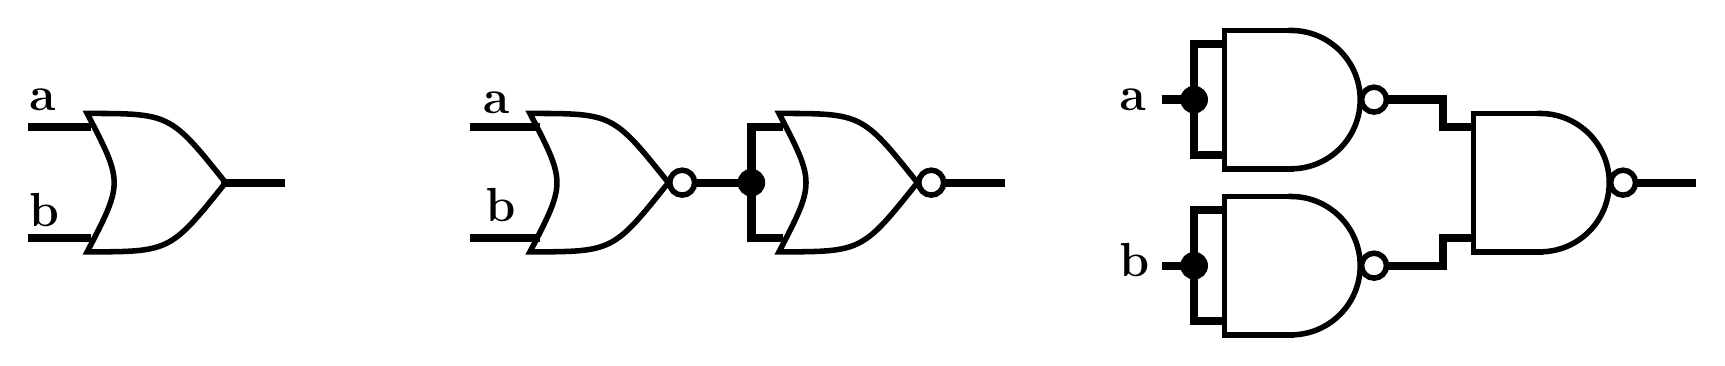
\begin{tikzpicture}[x=1pt,y=-1pt,line cap=rect]
\def\logisimfontA#1{\fontfamily{cmr}{#1}} % Replaced by logisim, original font was "SansSerif"
\definecolor{custcol_0_0_0}{RGB}{0, 0, 0}
\definecolor{custcol_ff_ff_ff}{RGB}{255, 255, 255}
\draw [line width=3.0pt, custcol_0_0_0 ]  (590.0,60.0) -- (610.0,60.0) ;
\draw [line width=3.0pt, custcol_0_0_0 ]  (250.0,60.0) -- (270.0,60.0) ;
\draw [line width=3.0pt, custcol_0_0_0 ]  (340.0,60.0) -- (360.0,60.0) ;
\draw [line width=3.0pt, custcol_0_0_0 ]  (80.0,60.0) -- (100.0,60.0) ;
\draw [line width=3.0pt, custcol_0_0_0 ]  (420.0,30.0) -- (430.0,30.0) ;
\draw [line width=3.0pt, custcol_0_0_0 ]  (440.0,10.0) -- (430.0,10.0) -- (430.0,30.0) -- (430.0,50.0) -- (440.0,50.0) ;
\draw [line width=3.0pt, custcol_0_0_0 ]  (420.0,90.0) -- (430.0,90.0) ;
\draw [line width=3.0pt, custcol_0_0_0 ]  (440.0,110.0) -- (430.0,110.0) -- (430.0,90.0) -- (430.0,70.0) -- (440.0,70.0) ;
\draw [line width=3.0pt, custcol_0_0_0 ]  (500.0,30.0) -- (520.0,30.0) -- (520.0,40.0) -- (530.0,40.0) ;
\draw [line width=3.0pt, custcol_0_0_0 ]  (500.0,90.0) -- (520.0,90.0) -- (520.0,80.0) -- (530.0,80.0) ;
\fill [line width=3.0pt, custcol_0_0_0]  (430.0,90.0) ellipse (5.0 and 5.0 );
\fill [line width=3.0pt, custcol_0_0_0]  (270.0,60.0) ellipse (5.0 and 5.0 );
\fill [line width=3.0pt, custcol_0_0_0]  (430.0,30.0) ellipse (5.0 and 5.0 );
\draw [line width=3.0pt, custcol_0_0_0 ]  (170.0,40.0) -- (190.0,40.0) -- (192.0,40.0) ;
\draw [line width=3.0pt, custcol_0_0_0 ]  (170.0,80.0) -- (190.0,80.0) -- (192.0,80.0) ;
\draw [line width=2.0pt, custcol_0_0_0 ]  (240.0,60.0) .. controls  (220.0,35.0)  ..  (190.0,35.0) .. controls  (203.0,60.0)  ..  (190.0,85.0) .. controls  (220.0,85.0)  ..  (240.0,60.0) -- cycle ;
\draw [line width=2.0pt, custcol_0_0_0]  (245.0,60.0) ellipse (4.5 and 4.5 );
\draw [line width=3.0pt, custcol_0_0_0 ]  (280.0,40.0) -- (280.0,40.0) -- (270.0,40.0) -- (270.0,60.0) -- (270.0,80.0) -- (280.0,80.0) -- (280.0,80.0) ;
\draw [line width=2.0pt, custcol_0_0_0 ]  (330.0,60.0) .. controls  (310.0,35.0)  ..  (280.0,35.0) .. controls  (293.0,60.0)  ..  (280.0,85.0) .. controls  (310.0,85.0)  ..  (330.0,60.0) -- cycle ;
\draw [line width=2.0pt, custcol_0_0_0]  (335.0,60.0) ellipse (4.5 and 4.5 );
\logisimfontA{\fontsize{16pt}{16pt}\fontseries{bx}\selectfont\node[inner sep=0, outer sep=0, custcol_0_0_0, anchor=base west] at  (9.0,34.0)  {a};}
\draw [line width=2.0pt, custcol_0_0_0] (555.0,85.0) arc (90.0:-90.0:25.0 and 25.0 );
\draw [line width=2.0pt, custcol_0_0_0 ]  (555.0,35.0) -- (531.0,35.0) -- (531.0,85.0) -- (555.0,85.0) ;
\draw [line width=2.0pt, custcol_0_0_0]  (585.0,60.0) ellipse (4.5 and 4.5 );
\logisimfontA{\fontsize{16pt}{16pt}\fontseries{bx}\selectfont\node[inner sep=0, outer sep=0, custcol_0_0_0, anchor=base west] at  (9.0,76.0)  {b};}
\logisimfontA{\fontsize{16pt}{16pt}\fontseries{bx}\selectfont\node[inner sep=0, outer sep=0, custcol_0_0_0, anchor=base west] at  (403.0,94.0)  {b};}
\logisimfontA{\fontsize{16pt}{16pt}\fontseries{bx}\selectfont\node[inner sep=0, outer sep=0, custcol_0_0_0, anchor=base west] at  (174.0,74.0)  {b};}
\logisimfontA{\fontsize{16pt}{16pt}\fontseries{bx}\selectfont\node[inner sep=0, outer sep=0, custcol_0_0_0, anchor=base west] at  (403.0,34.0)  {a};}
\draw [line width=2.0pt, custcol_0_0_0] (465.0,115.0) arc (90.0:-90.0:25.0 and 25.0 );
\draw [line width=2.0pt, custcol_0_0_0 ]  (465.0,65.0) -- (441.0,65.0) -- (441.0,115.0) -- (465.0,115.0) ;
\draw [line width=2.0pt, custcol_0_0_0]  (495.0,90.0) ellipse (4.5 and 4.5 );
\draw [line width=3.0pt, custcol_0_0_0 ]  (10.0,40.0) -- (30.0,40.0) -- (30.0,40.0) ;
\draw [line width=3.0pt, custcol_0_0_0 ]  (10.0,80.0) -- (30.0,80.0) -- (30.0,80.0) ;
\draw [line width=2.0pt, custcol_0_0_0 ]  (80.0,60.0) .. controls  (60.0,35.0)  ..  (30.0,35.0) .. controls  (43.0,60.0)  ..  (30.0,85.0) .. controls  (60.0,85.0)  ..  (80.0,60.0) -- cycle ;
\logisimfontA{\fontsize{16pt}{16pt}\fontseries{bx}\selectfont\node[inner sep=0, outer sep=0, custcol_0_0_0, anchor=base west] at  (173.0,35.0)  {a};}
\draw [line width=2.0pt, custcol_0_0_0] (465.0,55.0) arc (90.0:-90.0:25.0 and 25.0 );
\draw [line width=2.0pt, custcol_0_0_0 ]  (465.0,5.0) -- (441.0,5.0) -- (441.0,55.0) -- (465.0,55.0) ;
\draw [line width=2.0pt, custcol_0_0_0]  (495.0,30.0) ellipse (4.5 and 4.5 );
\end{tikzpicture}
}

		\label{fig:nandor}
	\end{figure}
\end{frame}

\section{O que mídia não quer que você saiba sobre o XOR \footnote[frame]{Coringando já...}}

\begin{frame}
	\frametitle{Equivalências do XOR}
	\par Até agora nos foram apresentadas as equivalências das portas AND e OR, porém, muitas vezes nos depararemos com portas XOR. Seria interessante sabermos sua equivalências também:
	
	\begin{table}[h!]
		\centering
		\begin{tabular}{|c|c|c|c|c|c|c|c|c|c|c|}
			\hline
			a & b & \(a \oplus b\) & \(\overline{a}b + a\overline{b}\) & \(\overline{\overline{a}\overline{b} + ab}\) & \(\overline{a}\) & \(\overline{b}\) & \(ab\) & \(\overline{a}b\) & \(a\overline{b}\) & \(\overline{a}\overline{b}\) \\ \hline
			0 & 0 & 0 & 0 & 0 & 1 & 1 & 0 & 0 & 0 & 1 \\ \hline
			0 & 1 & 1 & 1 & 1 & 1 & 0 & 0 & 1 & 0 & 0 \\ \hline
			1 & 0 & 1 & 1 & 1 & 0 & 1 & 0 & 0 & 1 & 0 \\ \hline
			1 & 1 & 0 & 0 & 0 & 0 & 0 & 1 & 0 & 0 & 0 \\ \hline
		\end{tabular}
		\caption{Tabela verdade das equivalências de XOR}
		\label{tab:equivalXOR}
	\end{table}
	
	\par $a \oplus b = \overline{a}b + a\overline{b}\ = \overline{\overline{a}\overline{b} + ab}$
	
\end{frame}

\begin{frame}
	\frametitle{Equivalências do XOR - Exercício}
	\par Usando a tabela verdade prove que $a \oplus (b \oplus c) = (a \oplus b) \oplus c$ e portanto que XOR é comutativo.
\end{frame}

\begin{frame}
	\frametitle{Revelação!}
	\par Que idade você tinha ao ficar sabendo que XOR só tem saída verdadeira quando o número de entradas verdadeiras é ímpar??
\end{frame}














